\let\negmedspace\undefined
\let\negthickspace\undefined
\documentclass[journal]{IEEEtran}
\usepackage[a5paper, margin=10mm, onecolumn]{geometry}
%\usepackage{lmodern} % Ensure lmodern is loaded for pdflatex
\usepackage{tfrupee} % Include tfrupee package

\setlength{\headheight}{1cm} % Set the height of the header box
\setlength{\headsep}{0mm}     % Set the distance between the header box and the top of the text

\usepackage{gvv-book}
\usepackage{gvv}
\usepackage{cite}
\usepackage{amsmath,amssymb,amsfonts,amsthm}
\usepackage{algorithmic}
\usepackage{graphicx}
\usepackage{textcomp}
\usepackage{xcolor}
\usepackage{txfonts}
\usepackage{listings}
\usepackage{enumitem}
\usepackage{mathtools}
\usepackage{gensymb}
\usepackage{comment}
\usepackage[breaklinks=true]{hyperref}
\usepackage{tkz-euclide} 
\usepackage{listings}
% \usepackage{gvv}                                        
\def\inputGnumericTable{}                                 
\usepackage[latin1]{inputenc}                                
\usepackage{color}                                            
\usepackage{array}                                            
\usepackage{longtable}                                       
\usepackage{calc}                                             
\usepackage{multirow}                                         
\usepackage{hhline}                                           
\usepackage{ifthen}                                           
\usepackage{lscape}
\begin{document}
\bibliographystyle{IEEEtran}
\title{2.7.14}
\author{EE25BTECH11002 - Achat Parth Kalpesh }
{\let\newpage\relax\maketitle}
\renewcommand{\thefigure}{\theenumi}
\renewcommand{\thetable}{\theenumi}
\setlength{\intextsep}{10pt} % Space between text and floats
\numberwithin{equation}{enumi}
\numberwithin{figure}{enumi}
\renewcommand{\thetable}{\theenumi}
\parindent 0px



\textbf{Question:}\\
If $\theta$ is the angle between the two vectors $\vec{a} = \hat{i} - 2\hat{j} + 3\hat{k}$ and $\vec{b} = 3\hat{i} - 2\hat{j} + \hat{k}$, find $\sin \theta$.

\textbf{Solution:}\\
Let the given vectors be represented by column matrices $\vec{a}$ and $\vec{b}$.
\begin{align}
    \vec{a} = \myvec{1 \\ -2 \\ 3}, \quad \vec{b} = \myvec{3 \\ -2 \\ 1}
\end{align}
The formula to calculate the angle $\sin\theta$ is given as,
\begin{align}
    \theta &= \cos^{-1}\brak{\frac{\abs{\vec{a}^\top\vec{b}}}{\norm{\vec{b}} \norm{\vec{a}}}}\\
    \sin\theta &= \sin\brak{\cos^{-1}\brak{\frac{\abs{\vec{a}^\top\vec{b}}}{\norm{\vec{a}} \norm{\vec{b}}}}}\\
    &= \sin\brak{\cos^{-1}\brak{\frac{\abs{\myvec{1&-2&3}\myvec{3\\-2\\1}}}{\norm{\myvec{1\\-2\\3}}\norm{\myvec{3\\-2\\1}}}}} \\
    &= \sin\brak{\cos^{-1} \brak{\frac{\abs{\brak{3}\brak{1} + \brak{-2}\brak{-2} + \brak{3}\brak{1}}}{\sqrt{1^2 + \brak{-2}^2 + 3^2}\sqrt{3^2 + \brak{-2}^2 + 1^2}}}} \\
    &= \sin\brak{\cos^{-1}\brak{\frac{\abs{3+4+3}}{\sqrt{14}\sqrt{14}}}}\\
    &= \sin\brak{\cos^{-1}\brak{\frac{10}{14}}}\\
    &= \frac{2\sqrt{6}}{7}
\end{align}
Therefore, the value of $\sin \theta$ is $\frac{2\sqrt{6}}{7}$.

\begin{figure}[h]
    \centering
    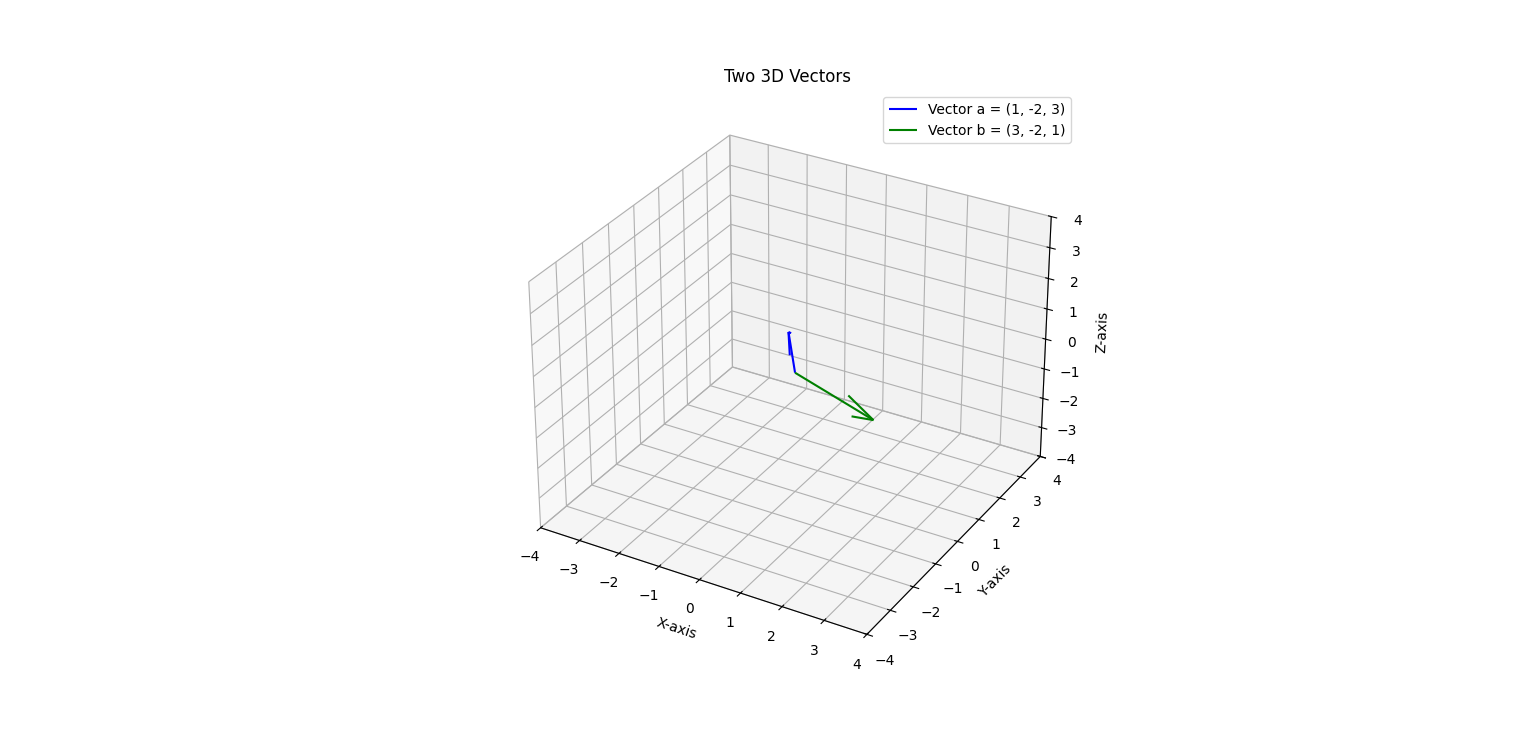
\includegraphics[width=\columnwidth]{figs/pure_python.png}
    \caption{Graph}
    \label{fig:fig}
 \end{figure}

\end{document}